% !TeX program = xelatex
% !TeX encoding = UTF-8
% 从项目根目录编译；正文、表格与图注均可直接编辑。
\documentclass[UTF8]{ctexart}
\usepackage[a4paper,left=17mm,right=17mm,top=15mm,bottom=15mm,includeheadfoot,headheight=16pt,headsep=5mm,footskip=8mm]{geometry}
\usepackage{graphicx,booktabs,array,tabularx}
\usepackage[unicode,hidelinks]{hyperref}
\hypersetup{pdftitle={软件工程实验二报告},pdfauthor={张博睿 241220007},pdfsubject={学校来宾酒店预订系统整体设计与界面设计},bookmarksnumbered=true}
\newcolumntype{Y}{>{\raggedright\arraybackslash}X}
% 全文固定A4纵向；分页只换页，不改变纸张尺寸。
\newcommand{\ReportPage}{\clearpage}
\title{软件工程实验二报告}
\author{张博睿\\学号：241220007}
\date{2026年11月6日}
\begin{document}
\pagenumbering{arabic}
\maketitle
\thispagestyle{empty}
\section*{目录}
\noindent\begin{tabularx}{\linewidth}{@{}p{15mm}Yp{23mm}@{}}
\toprule
部分 & 内容 & 起始页 \\
\midrule
一 & 主要功能 & \pageref{part:main} \\
二 & UML图 & \pageref{part:uml} \\
三 & UI界面 & \pageref{part:ui} \\
四 & 大模型使用 & \pageref{part:llm} \\
\bottomrule
\end{tabularx}

\ReportPage
\section{主要功能}\label{part:main}
系统面向本校来宾接待，连接学校接待人员、酒店工作人员、平台管理员和来宾四类用户。业务覆盖需求录入、酒店推荐、自动预订、住宿履约及异常安置；数据按接待责任和酒店归属隔离。文中的学校管理员与平台管理员指同一角色。

\subsubsection*{功能模块}
{
\noindent\begin{tabularx}{\linewidth}{@{}>{\bfseries}p{29mm}Y@{}}
\toprule
\textbf{模块} & \textbf{主要功能} \\
\midrule
身份与权限 & 四类用户登录，按角色、接待责任和酒店归属控制资料与操作范围。 \\
酒店与校方资料 & 维护酒店、接待地点、核实距离、学校审核评价及约定费用规则。 \\
房源管理 & 逐日维护房型价格、学校名额、确认占用、维修扣减和停售。 \\
查询与推荐 & 按日期、人数、房型、价格和距离筛选，结合价格、距离及评价排序。 \\
订单管理 & 录入需求、整单预订、查询结果、状态跟踪、改订和整单取消。 \\
入住与退房 & 逐人入住与补登记，办理续住、正常及提前退房、晚到与未入住。 \\
异常安置 & 酒店停业时保留原单和占用，确认替代新单后关闭原单并关联。 \\
通知与待处理 & 记录停业双渠道通知、未到店核实和未入住结果，跟进失败与确认待办。 \\
统计报表 & 按下单、计划住宿或实际住宿日期汇总人次、间夜及分类费用。 \\
操作日志 & 按权限追溯操作者、时间、对象和结果，记录异常处理及越权尝试。 \\
\bottomrule
\end{tabularx}\par
}
\subsubsection*{流程与规则}
业务依次完成需求录入、酒店筛选、方案确认、入住调整和退房统计。同酒店、同住宿日期可多房型合单；候选须已审核、学校评价至少70分、全部住宿晚有房，并符合预算和距离。

预订逐晚复核并锁定价格与规则。方案变化须重新确认，房源不足整单失败，同一请求不重复下单。改订失败保留原单；入住前一日18:00整起，特殊改订须管理员与酒店均确认。

取消、未入住及提前退房额外费用独立记录、线下结算。晚到先核实，未入住由酒店登记；停业替代成功后才关闭释放原单，并保留已住事实与费用。


\ReportPage
\section{UML图}\label{part:uml}
\subsubsection*{设计概览}
本设计使用PlantUML默认格式绘制五种、六张UML图，覆盖结构、行为和交互三类。以下按“模块与数据—角色与状态—关键业务交互”组织，分别说明系统如何划分、由谁操作以及如何保证处理顺序。

{
\noindent\begin{tabularx}{\linewidth}{@{}p{18mm}p{45mm}Y@{}}
\toprule
\textbf{分类} & \textbf{图形} & \textbf{主要表达内容} \\
\midrule
结构 & 组件图、类图 & 明确模块依赖、领域对象及数据关联。 \\
行为 & 用例图、状态图 & 界定四类用户的权限、业务目标及九种订单状态。 \\
交互 & 自动预订、停业安置序列图 & 描述方案复核、重复请求与新旧订单的一致处理。 \\
\bottomrule
\end{tabularx}\par
}
图形与UI遵循同一规则：普通预订自动确认；特殊改订须双方批准当前方案，再由接待人员确认差额；停业仅在替代新单成功后关闭释放原单。通知失败不撤销已提交业务。


% UML组1
\ReportPage
\phantomsection\pdfbookmark[1]{2.1 组件图}{uml-group-1}
\subsection*{2.1 组件图}
系统分为十个逻辑模块。查询与订单依赖酒店、房源数据，入住与安置处理住宿变化；权限、通知、统计和日志为业务提供支撑。订单、名额和请求结果保持一致，通知失败进入待处理。

\begin{center}
\centering
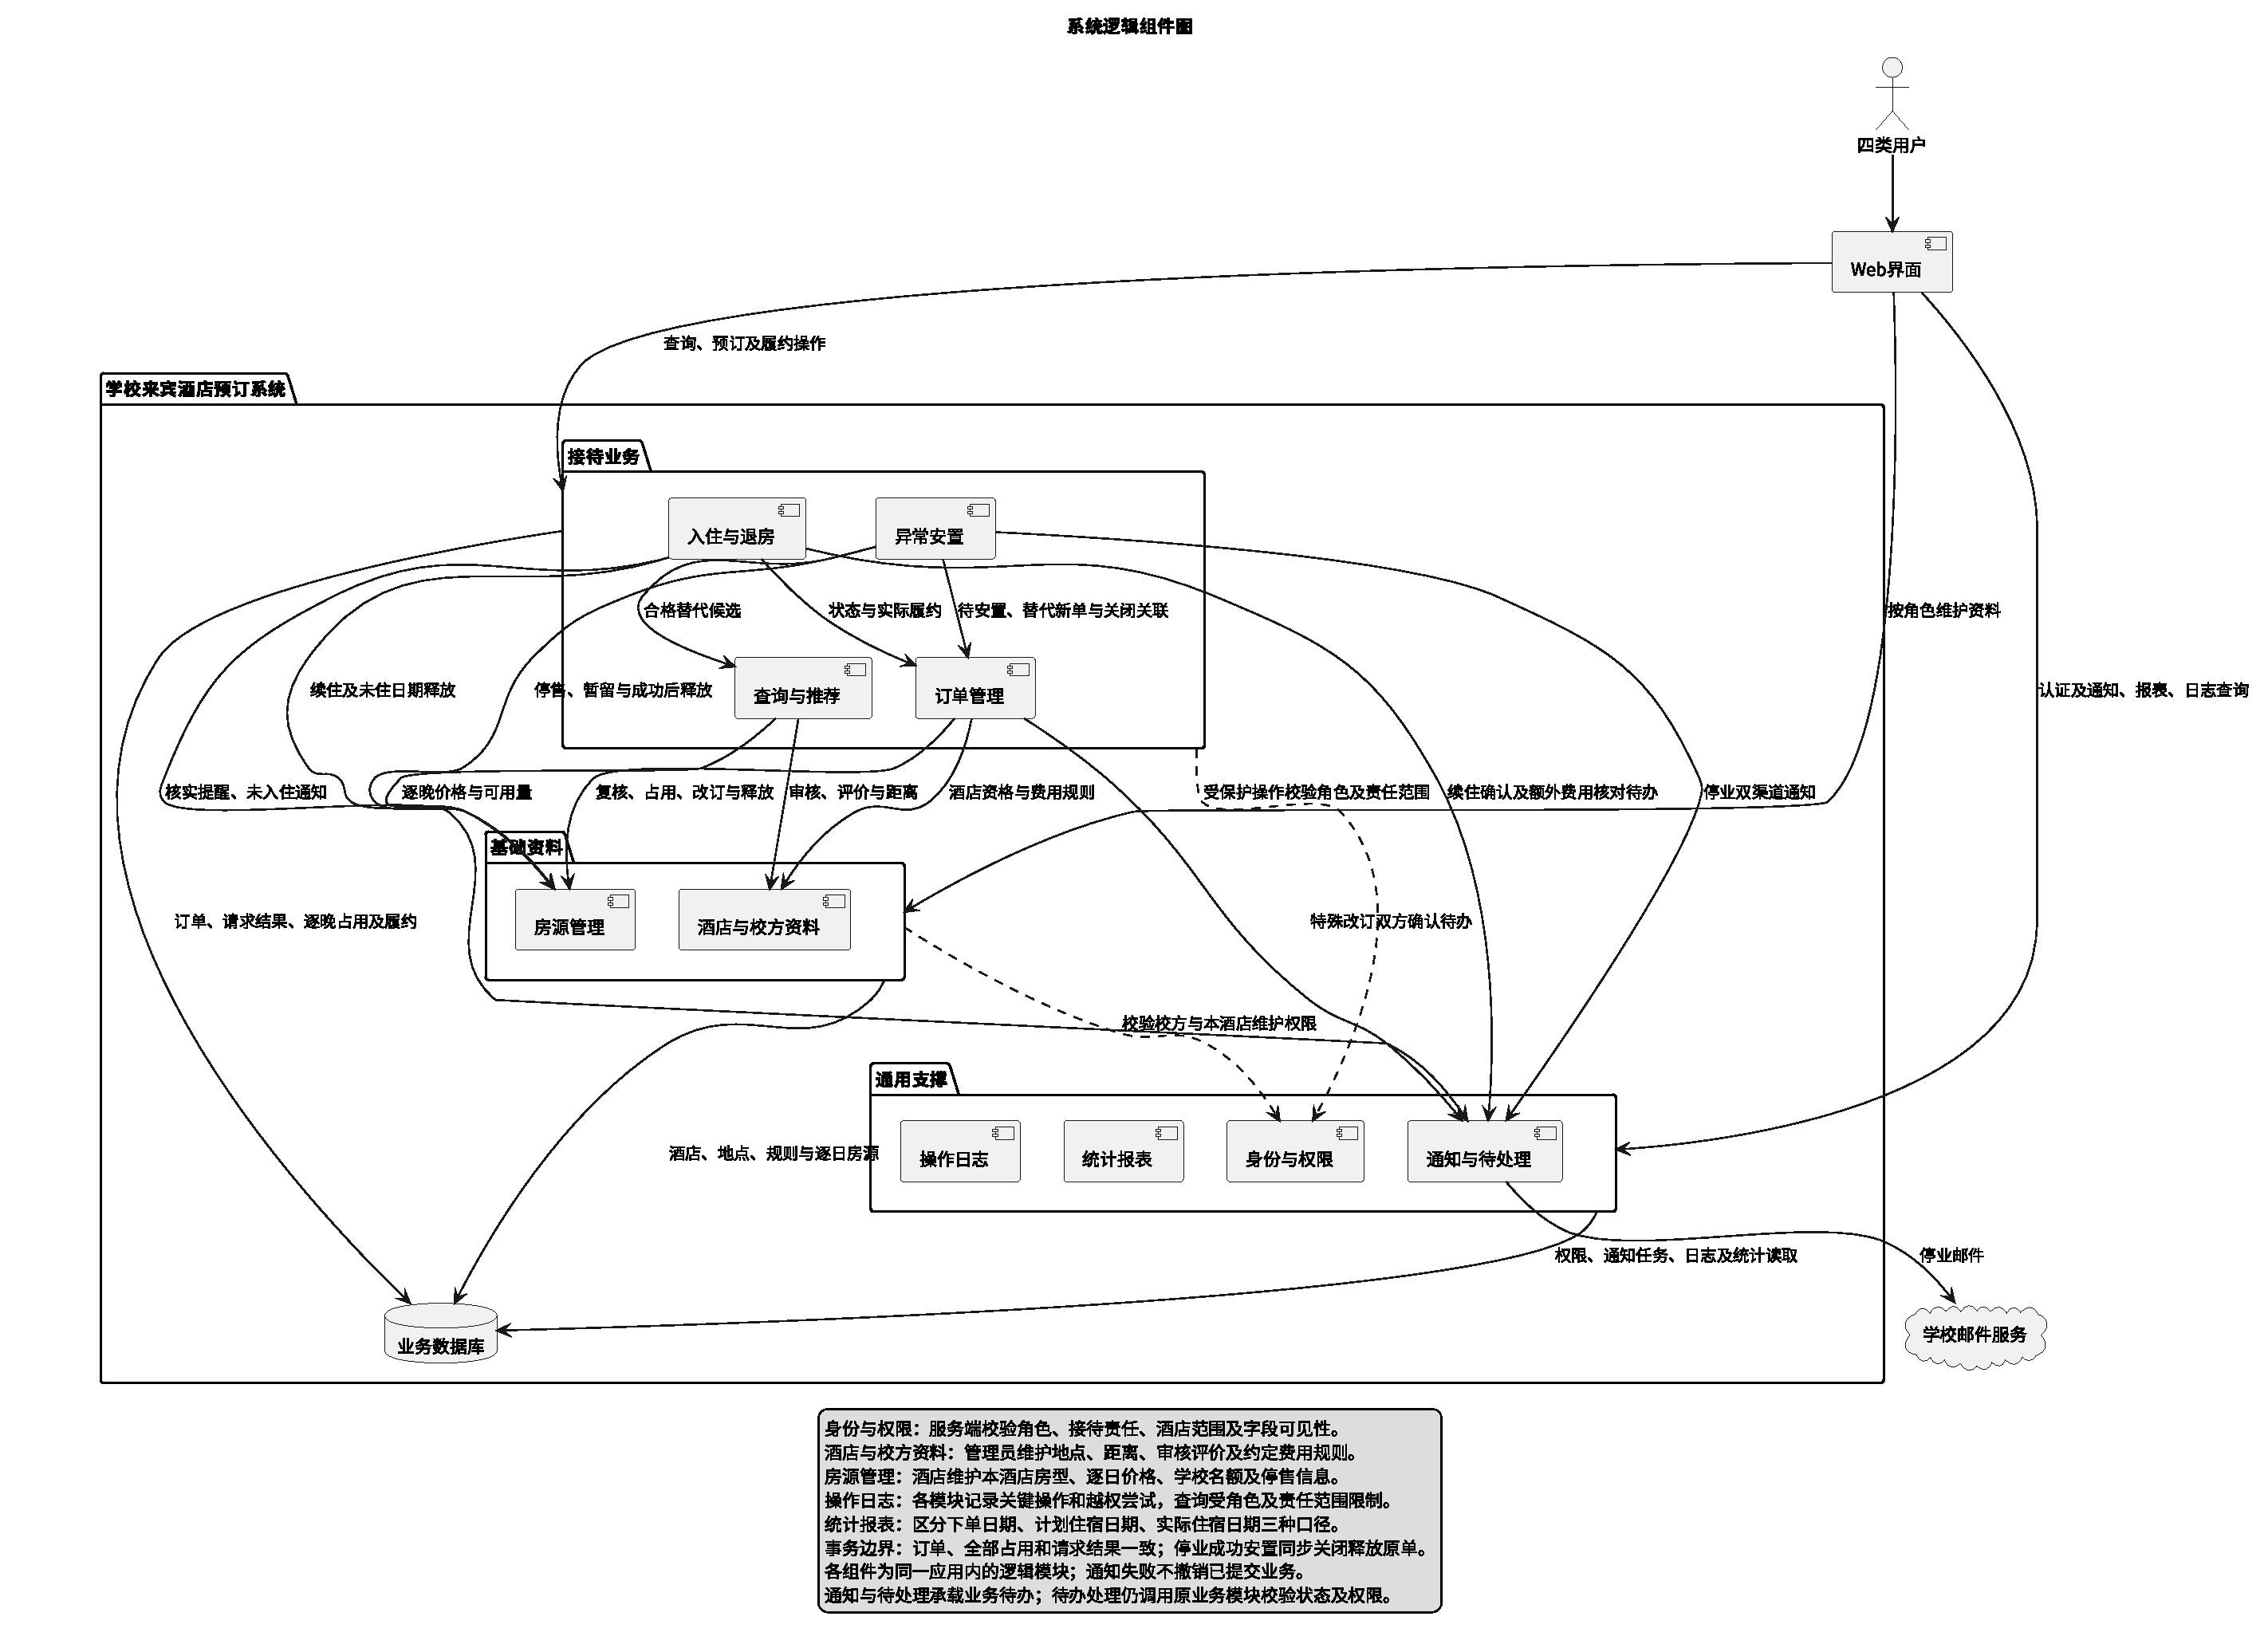
\includegraphics[page=1,width=\linewidth,height=180mm,keepaspectratio]{uml/uml-figures.pdf}
\par\smallskip
{图2-1 组件图\par}
\end{center}

% UML组2
\ReportPage
\phantomsection\pdfbookmark[1]{2.2 类图}{uml-group-2}
\subsection*{2.2 类图}
数据分为用户与需求、酒店与房源、订单与履约三组。订单包含房型及逐晚明细，并保存锁定价格和规则快照；入住记录按人登记，间夜按房间及日期统计。停业记录关联原单与替代新单，特殊改订记录绑定具体方案。

\begin{center}
\centering
\includegraphics[page=2,width=\linewidth,height=185mm,keepaspectratio]{uml/uml-figures.pdf}
\par\smallskip
{图2-2 类图\par}
\end{center}

% UML组3
\ReportPage
\phantomsection\pdfbookmark[1]{2.3 用例图}{uml-group-3}
\subsection*{2.3 用例图}
来宾查看本人安排，接待人员代订并处理负责订单，酒店管理本店房源和履约，管理员维护校方资料与规则。普通预订自动确认；特殊改订须管理员、酒店分别确认，再由接待人员确认方案和差额。

\begin{center}
\centering
\includegraphics[page=3,width=\linewidth,height=200mm,keepaspectratio]{uml/uml-figures.pdf}
\par\smallskip
{图2-3 用例图\par}
\end{center}

% UML组4
\ReportPage
\phantomsection\pdfbookmark[1]{2.4 订单状态}{uml-group-4}
\subsection*{2.4 订单状态}
订单共九种状态。改订成功保持已确认，补登记和续住保持已入住；终态不能恢复入住。替代新单确认成功前，原单保持待安置并保留占用。待重新确认属于请求进度，不另设订单状态。

\begin{center}
\centering
\includegraphics[page=4,width=\linewidth,height=195mm,keepaspectratio]{uml/uml-figures.pdf}
\par\smallskip
{图2-4 订单状态\par}
\end{center}

% UML组5
\ReportPage
\phantomsection\pdfbookmark[1]{2.5 自动预订}{uml-group-5}
\subsection*{2.5 自动预订}
先校验权限并查重，再复核酒店资格、规则、价格和逐晚名额。方案变化须重新确认，条件不满足则整单失败；成功时一致保存订单、占用和请求结果。响应不明确时查验原请求，避免重复预订。

\begin{center}
\centering
\includegraphics[page=5,width=\linewidth,height=200mm,keepaspectratio]{uml/uml-figures.pdf}
\par\smallskip
{图2-5 自动预订\par}
\end{center}

% UML组6
\ReportPage
\phantomsection\pdfbookmark[1]{2.6 停业安置}{uml-group-6}
\subsection*{2.6 停业安置}
停业后停售受影响日期，原单转待安置并保留占用，记录实住与费用并通知接待人员。替代仅覆盖剩余日期，复核原条件、报价及逐晚名额，方案变化须重新确认；新单确认、旧单关闭、占用释放与关联一并完成。失败保留原单，通知失败转管理员待处理，停售不随占用释放解除。

\begin{center}
\centering
\includegraphics[page=6,width=\linewidth,height=200mm,keepaspectratio]{uml/uml-figures.pdf}
\par\smallskip
{图2-6 停业安置\par}
\end{center}

\ReportPage
\section{UI界面}\label{part:ui}
\subsubsection*{设计思路}
使用Pixso将界面整合为8个1440×1000主界面，分别对应角色登录、平台管理、房源维护、住宿预订、订单与安置、入住与到店处理、住宿统计和来宾本人住宿。管理员、接待人员和酒店人员使用各自的导航，来宾只查看本人安排。深蓝导航、浅灰背景及白色卡片保持统一，关键状态同时用颜色和文字表达。

功能相近的页面合并到同一工作区：需求录入与酒店推荐合并，晚到核实并入入住处理，停业替代并入订单管理。账号、审核、房型编辑、方案确认、改订审批、通知及日志等次级功能保留按钮或菜单入口，不再分别展示完整页面。入口的可见范围及后续操作仍受角色、责任范围和酒店归属约束。

\subsubsection*{功能分布}
\noindent\begin{tabularx}{\linewidth}{@{}p{36mm}Y@{}}
\toprule
\textbf{主界面} & \textbf{主要功能与操作} \\
\midrule
角色登录 & 四类角色入口及账号登录。 \\
平台管理 & 酒店目录；酒店、地点、审核、费用规则、账号权限、通知待办及审计入口。 \\
每日房源与价格 & 逐晚价格、学校名额、占用、维修与停售；房型管理和酒店停业入口。 \\
住宿预订 & 住宿条件、来宾与房型摘要、候选酒店及排序；资料编辑和方案确认入口。 \\
订单与安置 & 订单状态、前后改订方案及差额；取消、续住确认、请求查询及停业替代入口。 \\
入住与到店处理 & 本店订单、逐人登记、续住与退房；晚到、未入住及酒店特殊改订确认入口。 \\
接待住宿统计 & 三种日期口径、人次、去重人数、间夜和分类费用；明细及导出入口。 \\
来宾本人住宿 & 本人酒店、日期、房型、状态与联系入口，隐藏协议价和他人信息。 \\
\bottomrule
\end{tabularx}

\subsubsection*{入口与规则}
入口表示后续功能的到达位置，不改变业务生效条件。普通预订自动确认；特殊改订须管理员与酒店批准当前版本，再由接待人员确认差额；续住须负责接待人员确认；未入住由酒店人工登记；停业替代成功后才关闭释放原单。通知失败只进入跟进，不撤销已完成业务。

\ReportPage
\phantomsection\pdfbookmark[1]{3.1 角色登录}{ui-screen-1}
\subsection*{3.1 角色登录}
\begin{center}
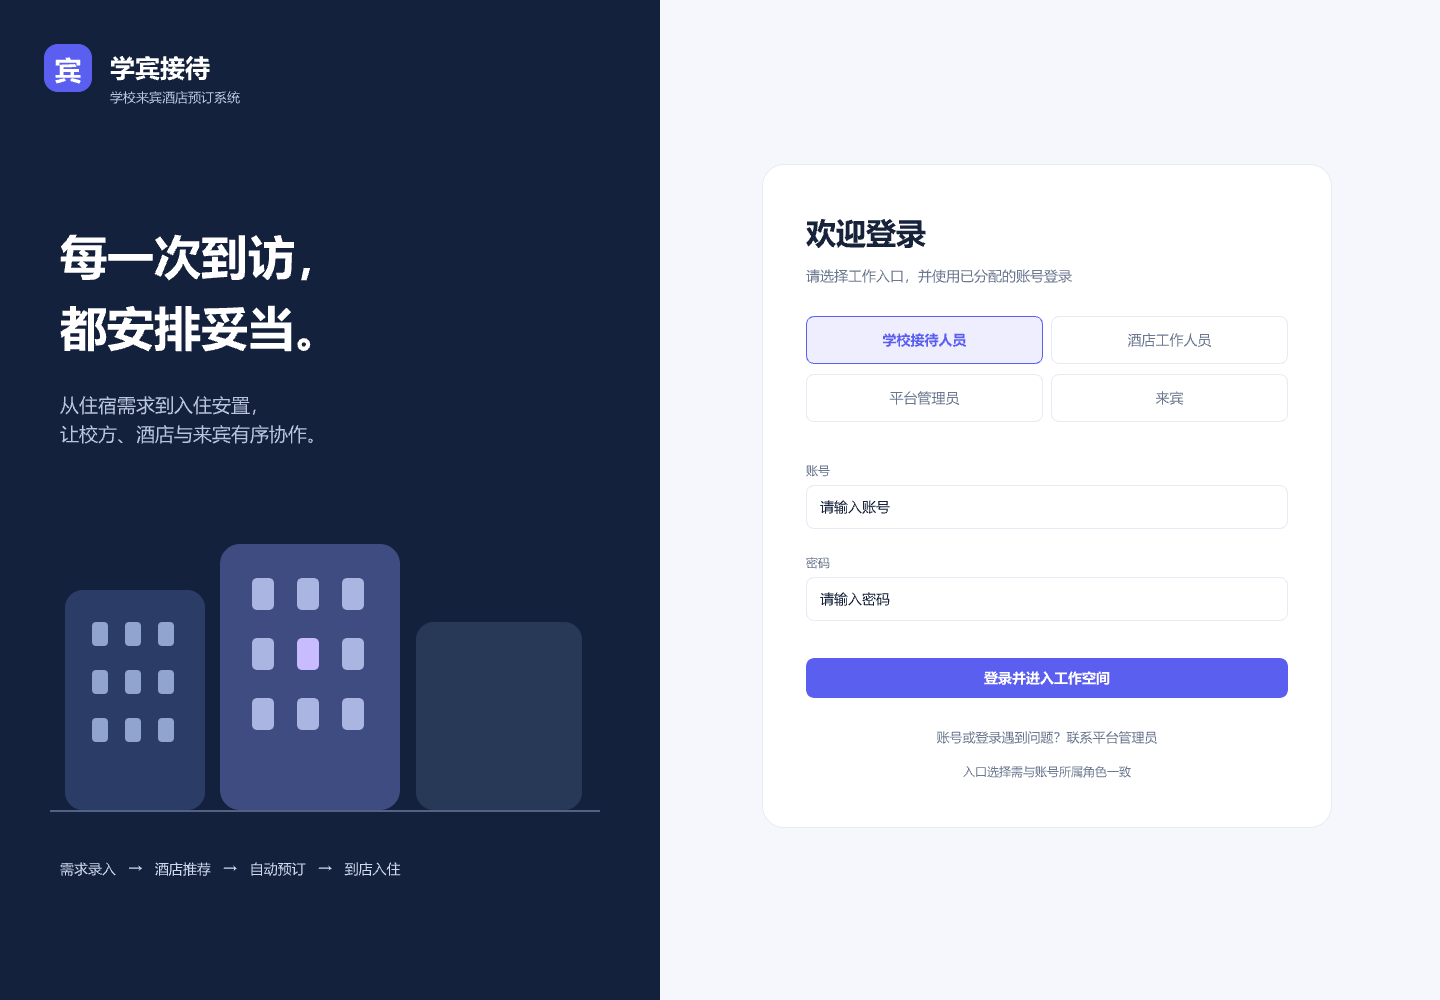
\includegraphics[width=\linewidth,height=130mm,keepaspectratio]{UI/UI角色登录.png}
\par\smallskip 图3-1 角色登录
\end{center}
\noindent\textbf{布局与操作：}左侧介绍接待流程，右侧集中四类角色入口、账号和密码。用户选择与账号相符的入口，登录后进入对应工作空间。

\noindent\textbf{权限规则：}入口选择不直接授予权限。接待人员限负责订单，酒店人员限本酒店，管理员按平台职责操作，来宾仅查看本人住宿。账号停用后不得继续执行受保护操作。

\ReportPage
\phantomsection\pdfbookmark[1]{3.2 平台管理}{ui-screen-2}
\subsection*{3.2 平台管理}
\begin{center}
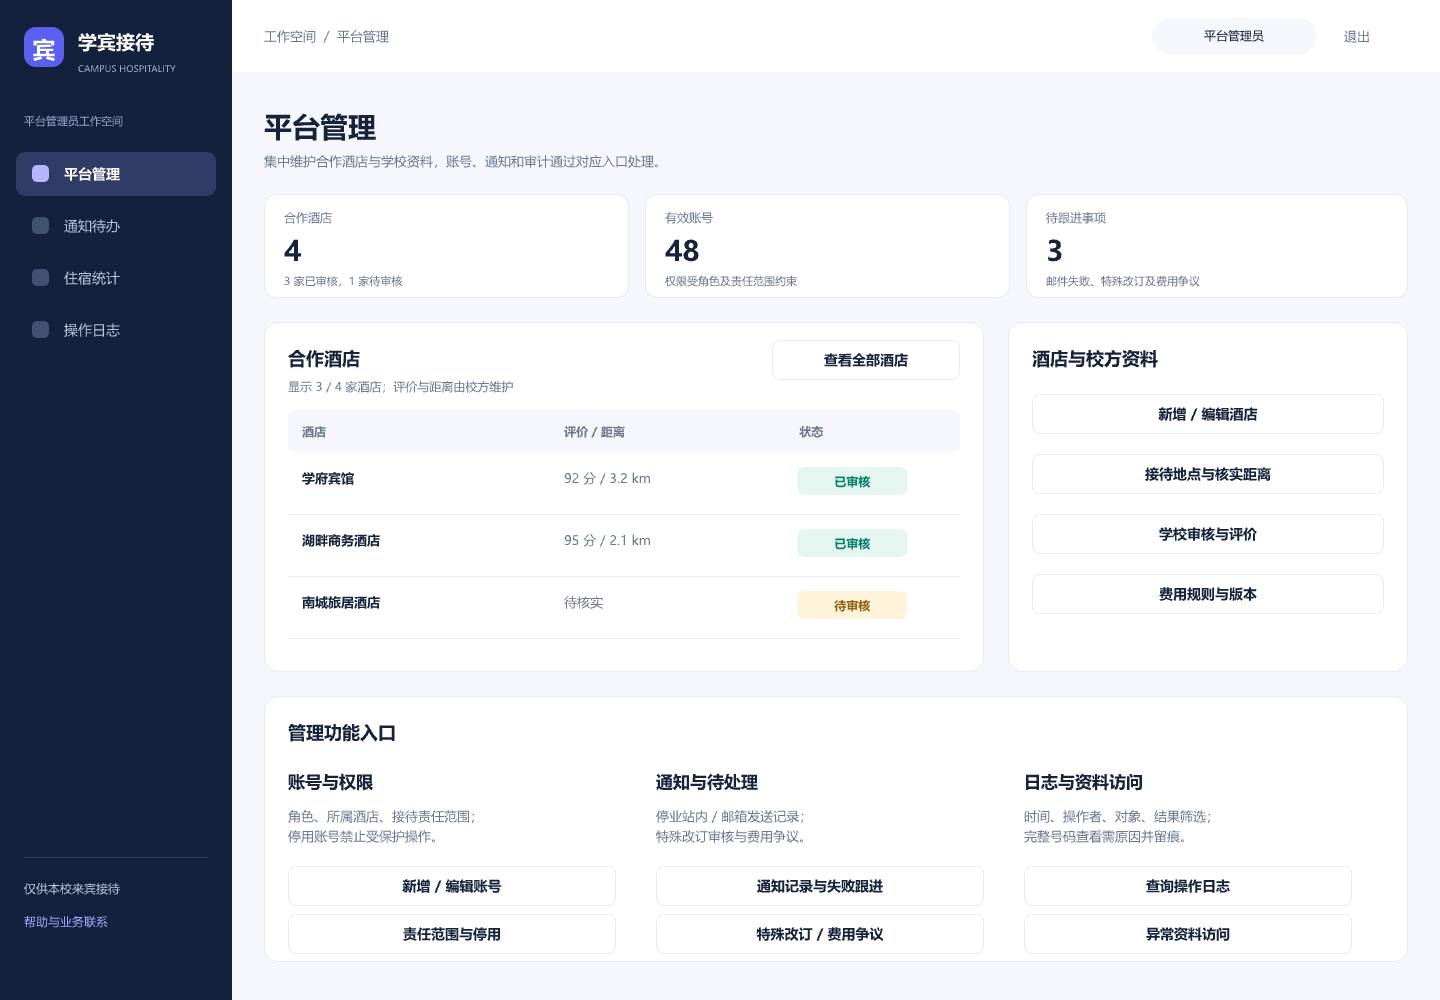
\includegraphics[width=\linewidth,height=130mm,keepaspectratio]{UI/UI平台管理.png}
\par\smallskip 图3-2 平台管理
\end{center}
\noindent\textbf{布局与操作：}上方汇总合作酒店、账号及待跟进事项，中部酒店目录标明当前显示3/4家，可通过“查看全部酒店”查看完整名单。右侧提供酒店档案编辑、接待地点与核实距离维护、学校审核评价及费用规则版本入口；下方集中账号及责任范围管理、通知发送记录与失败跟进、特殊改订审核、费用争议处理、日志查询及异常资料访问。

\noindent\textbf{规则：}校方维护质量依据，已审核且评价至少70分才能参与预订。订单保存确认时的费用规则；管理员默认查看脱敏号码，处理具体异常时需填写原因并留痕。

\ReportPage
\phantomsection\pdfbookmark[1]{3.3 每日房源与价格}{ui-screen-3}
\subsection*{3.3 每日房源与价格}
\begin{center}
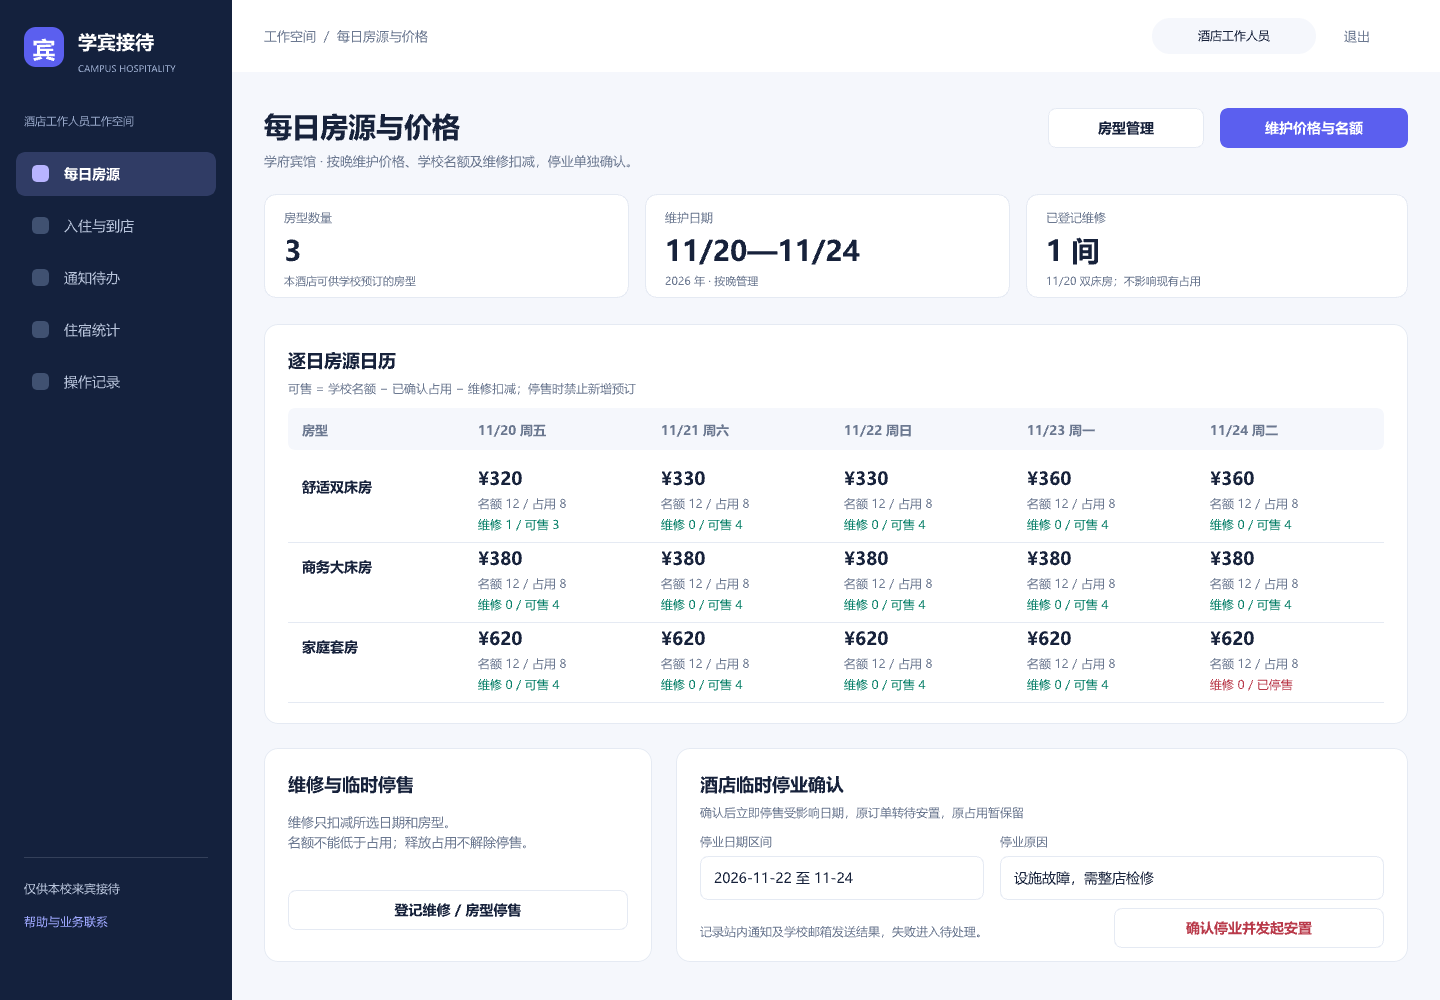
\includegraphics[width=\linewidth,height=130mm,keepaspectratio]{UI/UI每日房源与价格.png}
\par\smallskip 图3-3 每日房源与价格
\end{center}
\noindent\textbf{布局与操作：}酒店人员按房型、日期查看逐晚价格、学校名额、已确认占用、维修扣减及可售量，通过页首入口新增或编辑房型、批量维护价格与名额。下方分别提供维修停售登记和整店停业确认，避免混淆两类处理。

\noindent\textbf{规则：}可售量为学校名额减去已确认占用及维修扣减，名额不得低于现有占用。停售禁止新增预订，释放占用不自动解除停售。酒店停业须确认受影响日期与原因，随后记录站内、学校邮箱两个通知结果，失败交管理员跟进。

\ReportPage
\phantomsection\pdfbookmark[1]{3.4 住宿预订}{ui-screen-4}
\subsection*{3.4 住宿预订}
\begin{center}
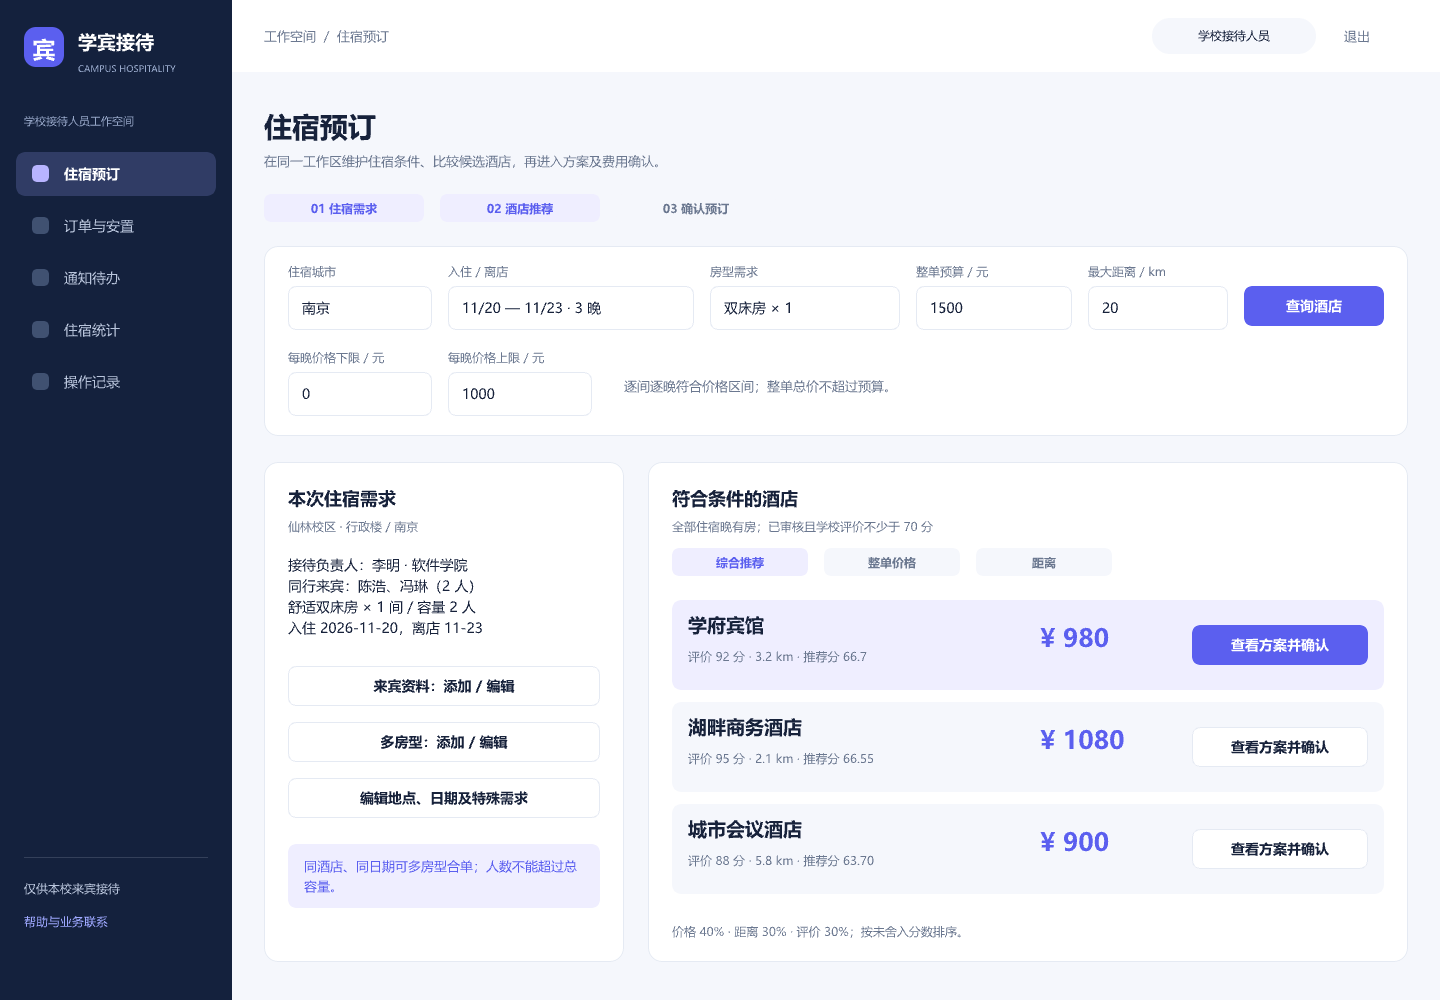
\includegraphics[width=\linewidth,height=130mm,keepaspectratio]{UI/UI住宿预订.png}
\par\smallskip 图3-4 住宿预订
\end{center}
\noindent\textbf{布局与操作：}顶部统一填写城市、日期、房型、整单预算、最大距离和每晚价格区间；左侧汇总来宾及住宿条件，并提供来宾、多房型、地点日期及特殊需求的添加或编辑入口；右侧比较候选酒店。通过所选酒店的“查看方案并确认”进入确认流程，核对逐晚价格、总价、取消期限及费用规则，并取得请求编号，衔接需求录入、查询推荐与预订确认。

\noindent\textbf{规则：}同酒店、同日期可多房型合单，人数不得超过容量。全部住宿晚均须可订；预算与最大距离为正，距离默认20公里。推荐分按价格40\%、距离30\%、评价30\%计算，按未舍入分数排序。提交时复核报价与名额，变化须重新确认，无房整单失败；普通预订自动确认。

\ReportPage
\phantomsection\pdfbookmark[1]{3.5 订单与安置}{ui-screen-5}
\subsection*{3.5 订单与安置}
\begin{center}
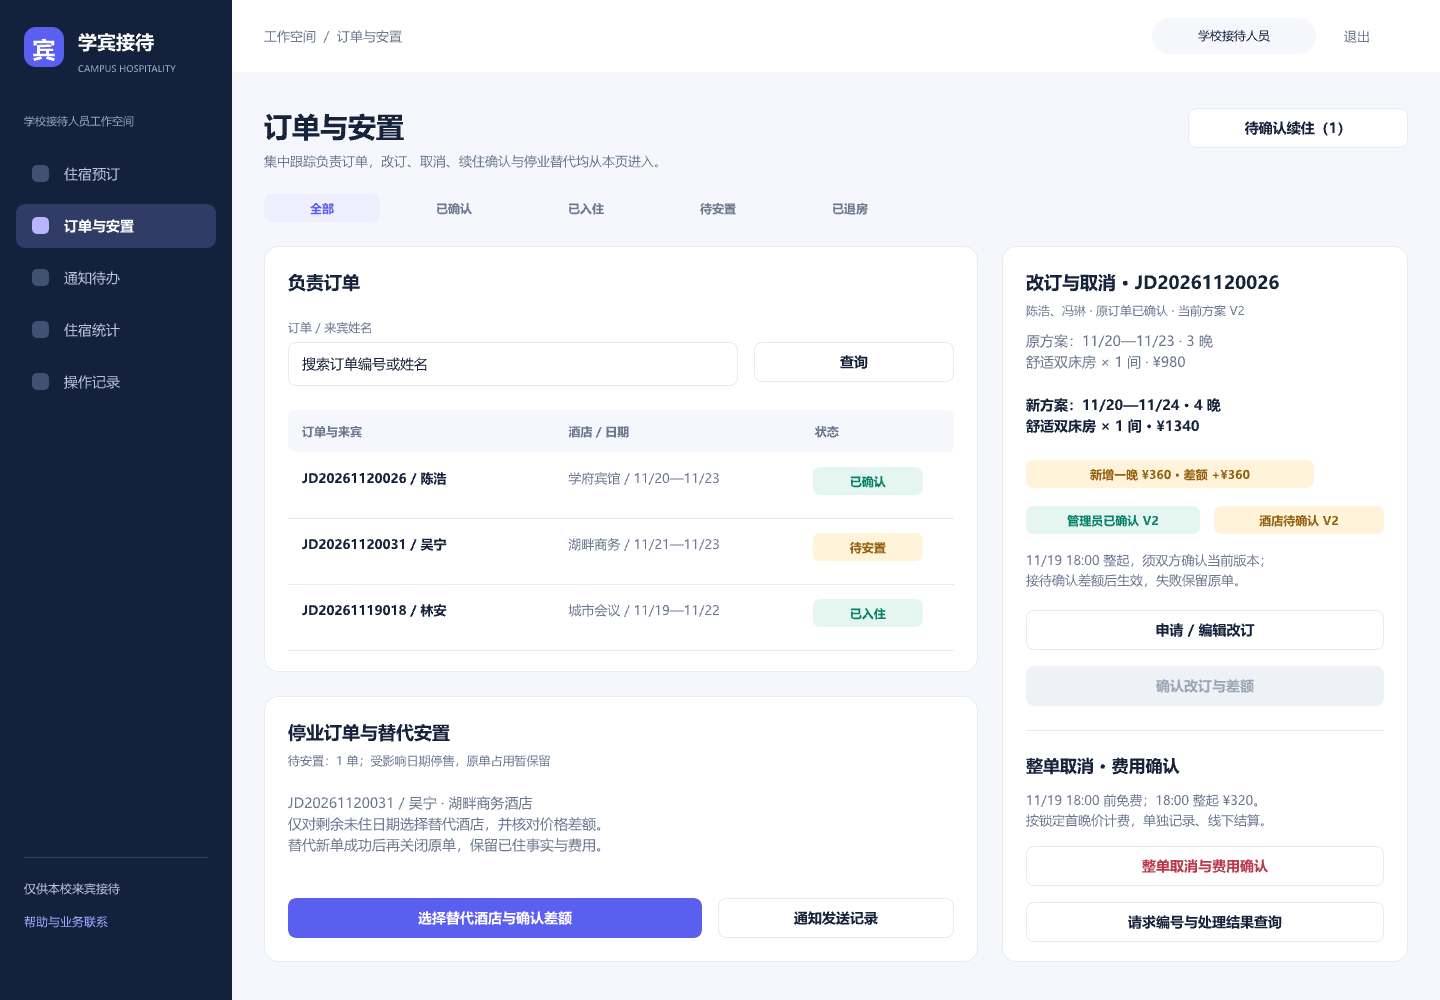
\includegraphics[width=\linewidth,height=130mm,keepaspectratio]{UI/UI订单与安置.png}
\par\smallskip 图3-5 订单与安置
\end{center}
\noindent\textbf{布局与操作：}左侧查询负责订单并处理停业待安置事项，通过相应按钮选择替代酒店、确认差额或查看通知发送记录；右侧对比改订前后的日期、房型、价格和差额，并提供改订申请编辑、整单取消费用确认及原请求编号与处理结果查询入口。页首“待确认续住”用于接待人员核对并确认续住申请。

\noindent\textbf{规则：}前一日18:00整起，特殊改订需管理员与酒店确认当前版本，再由接待确认差额。任一批准缺失时确认按钮禁用，修改方案使旧批准失效。取消前展示费用，18:00整起按各间锁定首晚价汇总、单列线下结算。停业只安置剩余日期；新单成功后才关闭原单、释放占用并建立关联，失败保留原单。

\ReportPage
\phantomsection\pdfbookmark[1]{3.6 入住与到店处理}{ui-screen-6}
\subsection*{3.6 入住与到店处理}
\begin{center}
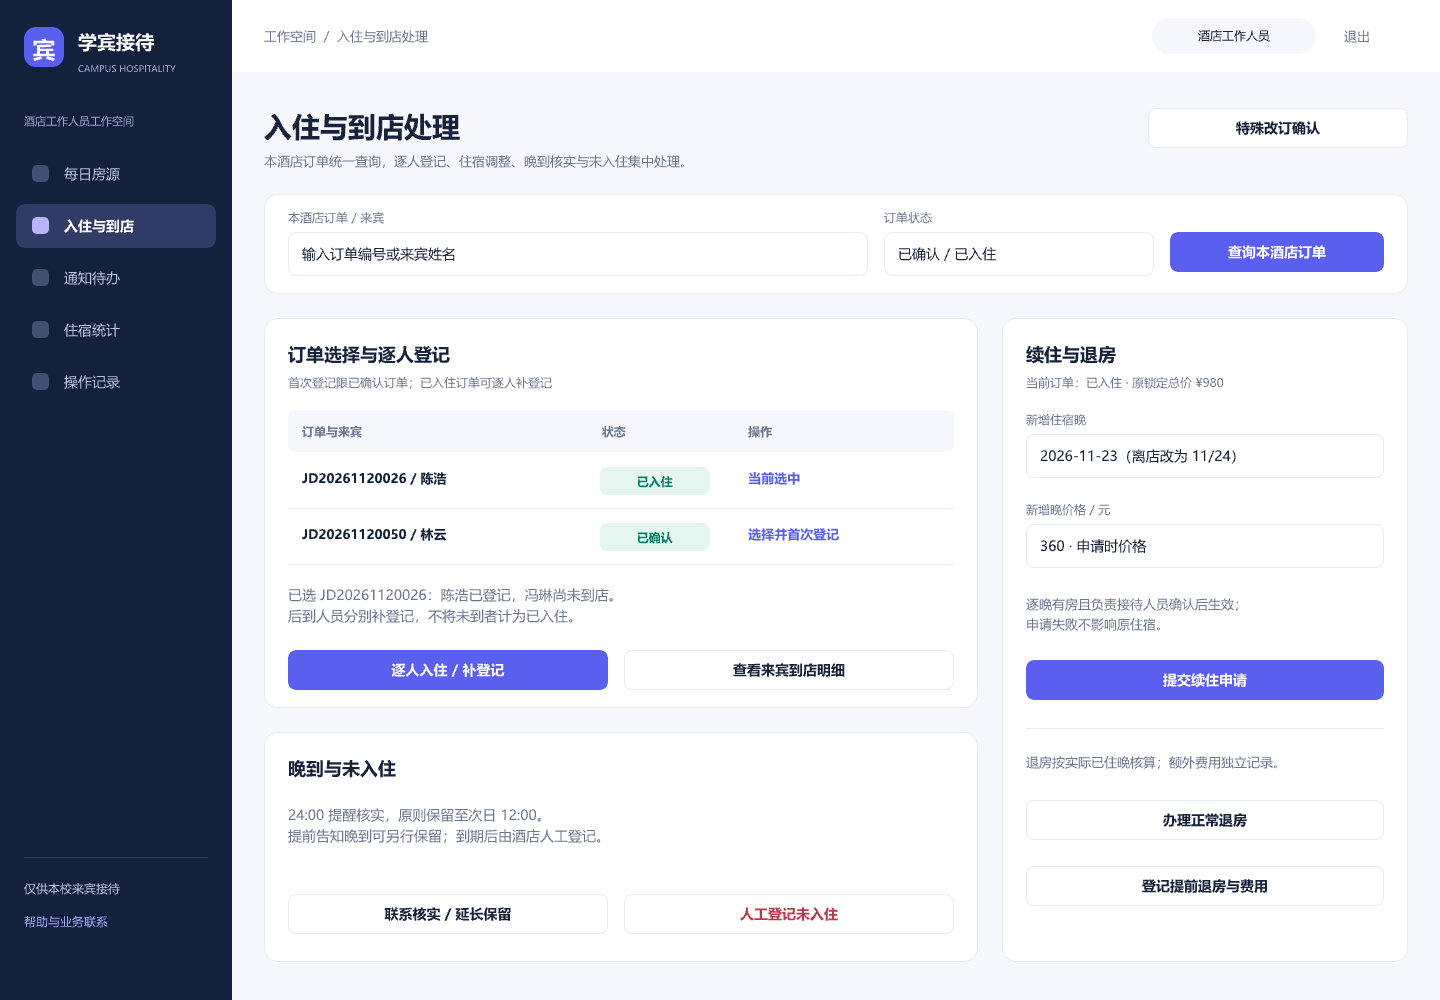
\includegraphics[width=\linewidth,height=130mm,keepaspectratio]{UI/UI入住与到店处理.png}
\par\smallskip 图3-6 入住与到店处理
\end{center}
\noindent\textbf{布局与操作：}顶部查询本酒店订单，页首提供酒店特殊改订确认入口；左侧选择订单，进入首次入住或补登记，并查看逐人到店明细；下方集中联系核实、另行保留和人工登记未入住入口；右侧提交续住申请、办理正常退房，或登记提前退房及额外费用。

\noindent\textbf{规则：}首位来宾登记后订单转已入住，未到者不计为入住。续住按申请时新增晚价格，由负责接待人员确认；提前退房只核算已住晚并释放未来名额，额外费用单列。计划入住日24:00提醒核实，原则保留到次日12:00；未入住须酒店人工登记，之后晚到须重新预订。

\ReportPage
\phantomsection\pdfbookmark[1]{3.7 接待住宿统计}{ui-screen-7}
\subsection*{3.7 接待住宿统计}
\begin{center}
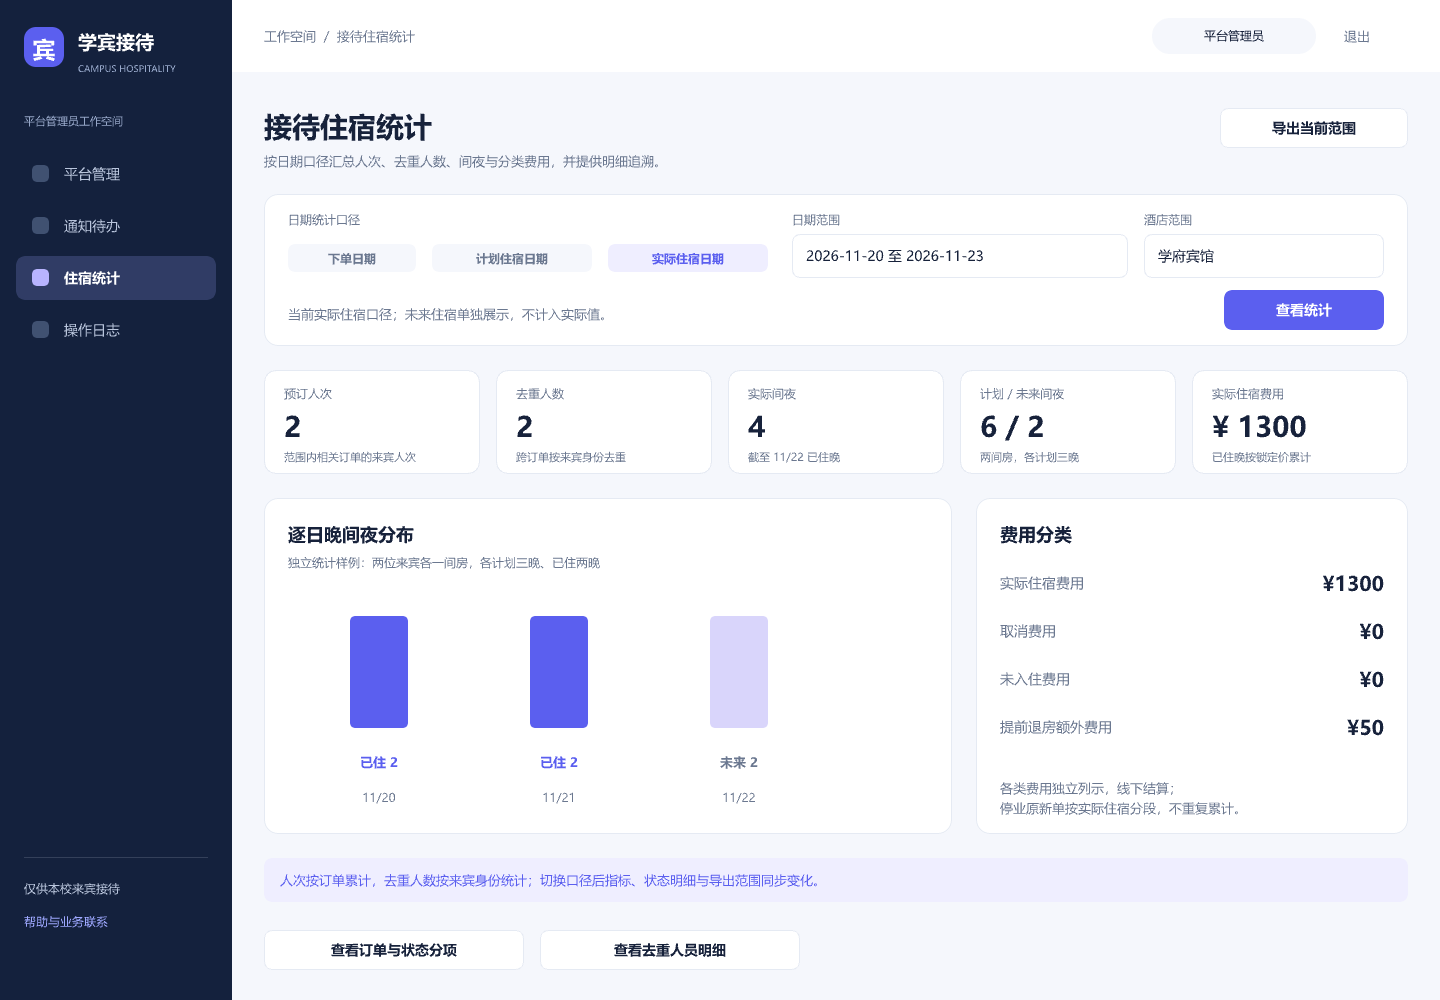
\includegraphics[width=\linewidth,height=130mm,keepaspectratio]{UI/UI接待住宿统计.png}
\par\smallskip 图3-7 接待住宿统计
\end{center}
\noindent\textbf{布局与操作：}按下单日期、计划住宿日期或实际住宿日期切换口径，并选择日期和酒店范围。人次、去重人数、实际间夜、计划与未来间夜、住宿费用直接展示，通过相应按钮查看订单状态分项、去重人员明细或导出当前范围。

\noindent\textbf{规则：}图中为独立统计样例：两位来宾各一间房、各计划三晚，已住两晚，共计划6间夜、实际4间夜、未来2间夜。实际住宿费用1300元，额外费用50元单列。未来住宿不计实际值，停业新旧单按实住分段、不重复累计。接待人员及酒店从各自菜单进入，仅查看职责范围内的统计。

\ReportPage
\phantomsection\pdfbookmark[1]{3.8 来宾本人住宿}{ui-screen-8}
\subsection*{3.8 来宾本人住宿}
\begin{center}
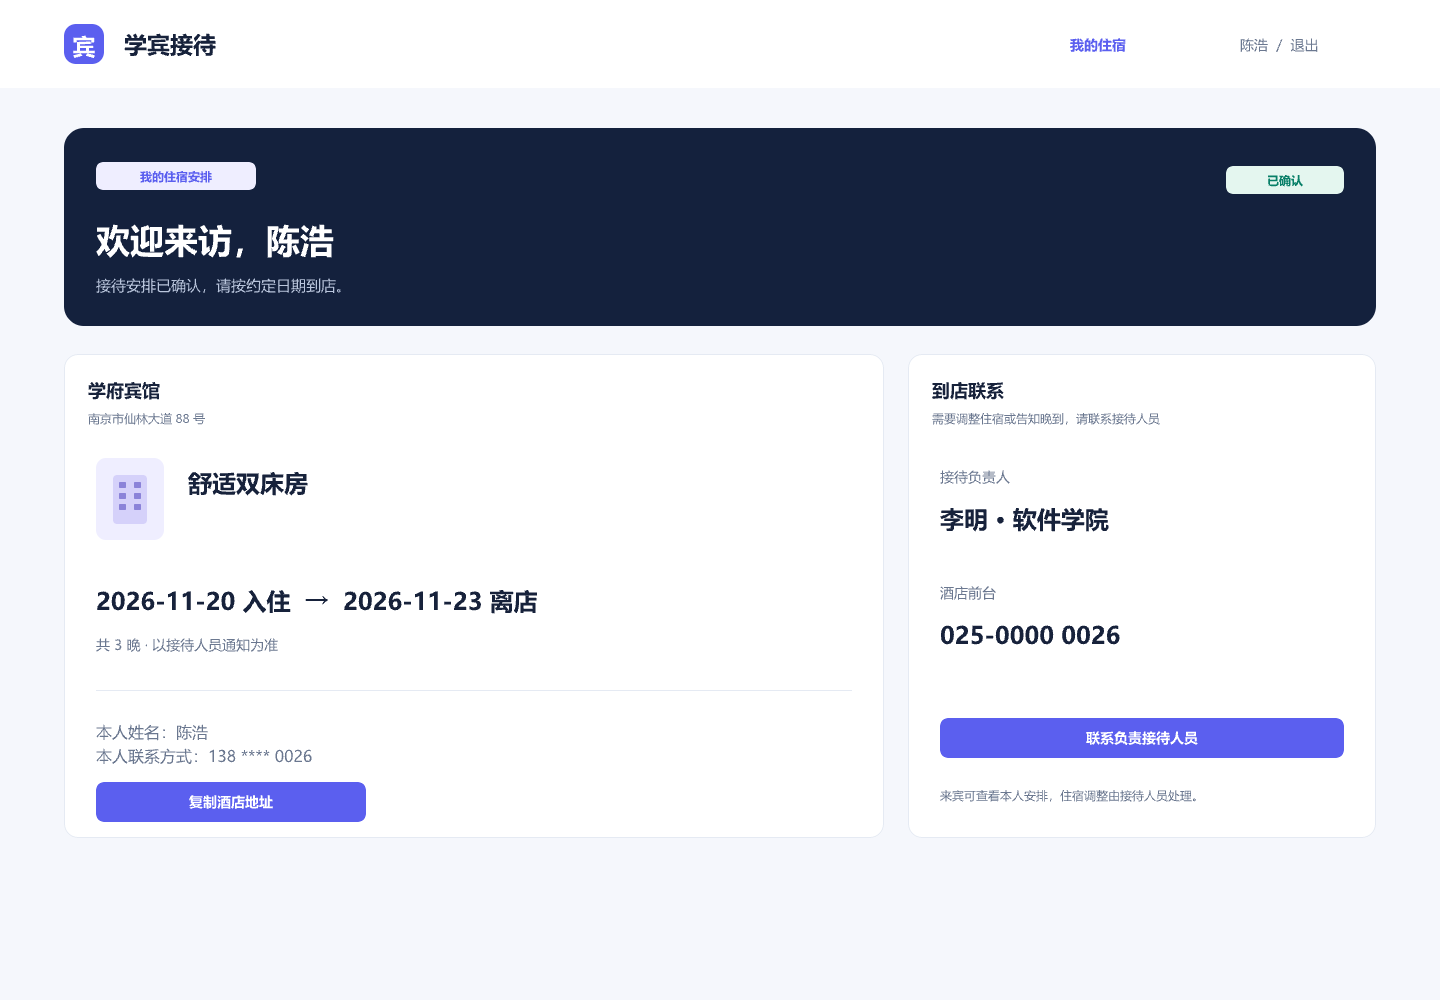
\includegraphics[width=\linewidth,height=130mm,keepaspectratio]{UI/UI来宾本人住宿.png}
\par\smallskip 图3-8 来宾本人住宿
\end{center}
\noindent\textbf{布局与操作：}集中展示本人酒店、地址、入住离店日期、房型、住宿状态及接待联系信息，保留复制地址和联系负责接待人员的入口。

\noindent\textbf{规则：}只显示本人住宿信息及脱敏联系方式，不展示协议价格、同单其他来宾资料或后台管理入口。住宿调整和晚到告知由负责接待人员协调，来宾不能直接修改订单。

\ReportPage
\section{大模型使用}\label{part:llm}

\phantomsection\pdfbookmark[1]{4.1 UML图}{llm-section-1}
\subsection*{4.1 UML图}
我将实验内容和requirements.md中的需求提供给ChatGPT，让其分析角色、功能与业务流程，生成组件图、类图、用例图、状态图及两张序列图的PlantUML代码，再使用PlantUML工具按默认格式渲染。

\textbf{人工检查是确认UML设计正确性的必要环节。}生成代码和图形后，需要由我对照实验内容与需求说明，逐项检查角色权限、对象关系、状态转换条件、交互顺序及异常分支，并核对各图之间是否一致。发现遗漏、歧义或矛盾时，应明确指出问题，修改PlantUML代码并重新渲染，再次人工复核。大模型输出只能作为待审核初稿，只有经过人工检查和修正，才能作为最终设计，不能直接依赖生成结果。

\phantomsection\pdfbookmark[1]{4.2 UI界面}{llm-section-2}
\subsection*{4.2 UI界面}
我让ChatGPT根据功能模块和用户角色提出导航、布局、配色及字段组织建议，再结合个人偏好调整，辅助我绘制界面。新版使用Pixso完成设计，并通过MCP连接将方案绘制为原生可编辑图层，导出PNG供报告使用。对照旧版与需求检查后，补齐首次入住、多房型、价格区间、请求编号、维修扣减、人次统计和日志时间范围等内容，并检查实际截图与文字说明。

Pixso是一款界面设计与协作工具，支持画板、矢量图形、文字、组件和原型连接，可以组织多个页面并导出图片。它便于统一视觉样式和继续编辑设计稿；本实验使用画板与原生图层表达页面结构、字段和操作状态。

\phantomsection\pdfbookmark[1]{4.3 思考与总结}{llm-section-3}
\subsection*{4.3 思考与总结}
性能较强的大模型能够基本胜任需求整理、图形代码生成和界面建议等作业任务，但仍可能遗漏操作入口、误解业务规则，或生成相互矛盾的内容。经过检查后可发现，输出完整并不代表设计正确。不能过度依赖大模型，生成内容需要人工检查，并结合工具运行结果验证；使用者应理解设计依据，最终由人判断需求、UML、UI和报告是否一致。

\label{report:last}
\end{document}
